%%%%%%%%%%%%  Generated using docx2latex.com  %%%%%%%%%%%%%%

%%%%%%%%%%%%  v2.0.0-beta  %%%%%%%%%%%%%%

\documentclass[12pt]{article}
\usepackage{amsmath}
\usepackage{latexsym}
\usepackage{amsfonts}
\usepackage[normalem]{ulem}
\usepackage{soul}
\usepackage{array}
\usepackage{amssymb}
\usepackage{extarrows}
\usepackage{graphicx}
\usepackage[backend=biber,
style=numeric,
sorting=none,
isbn=false,
doi=false,
url=false,
]{biblatex}\addbibresource{bibliography.bib}

\usepackage{subfig}
\usepackage{wrapfig}
\usepackage{wasysym}
\usepackage{enumitem}
\usepackage{adjustbox}
\usepackage{ragged2e}
\usepackage[svgnames,table]{xcolor}
\usepackage{tikz}
\usepackage{longtable}
\usepackage{changepage}
\usepackage{setspace}
\usepackage{hhline}
\usepackage{multicol}
\usepackage{tabto}
\usepackage{float}
\usepackage{multirow}
\usepackage{makecell}
\usepackage{fancyhdr}
\usepackage[toc,page]{appendix}
\usepackage[hidelinks]{hyperref}
\usetikzlibrary{shapes.symbols,shapes.geometric,shadows,arrows.meta}
\tikzset{>={Latex[width=1.5mm,length=2mm]}}
\usepackage{flowchart}\usepackage[paperheight=11.69in,paperwidth=8.26in,left=1.0in,right=1.0in,top=1.0in,bottom=1.0in,headheight=1in]{geometry}
\usepackage[utf8]{inputenc}
\usepackage[T1]{fontenc}
\TabPositions{0.5in,1.0in,1.5in,2.0in,2.5in,3.0in,3.5in,4.0in,4.5in,5.0in,5.5in,6.0in,}

\urlstyle{same}


 %%%%%%%%%%%%  Set Depths for Sections  %%%%%%%%%%%%%%

% 1) Section
% 1.1) SubSection
% 1.1.1) SubSubSection
% 1.1.1.1) Paragraph
% 1.1.1.1.1) Subparagraph


\setcounter{tocdepth}{5}
\setcounter{secnumdepth}{5}


 %%%%%%%%%%%%  Set Depths for Nested Lists created by \begin{enumerate}  %%%%%%%%%%%%%%


\setlistdepth{9}
\renewlist{enumerate}{enumerate}{9}
		\setlist[enumerate,1]{label=\arabic*)}
		\setlist[enumerate,2]{label=\alph*)}
		\setlist[enumerate,3]{label=(\roman*)}
		\setlist[enumerate,4]{label=(\arabic*)}
		\setlist[enumerate,5]{label=(\Alph*)}
		\setlist[enumerate,6]{label=(\Roman*)}
		\setlist[enumerate,7]{label=\arabic*}
		\setlist[enumerate,8]{label=\alph*}
		\setlist[enumerate,9]{label=\roman*}

\renewlist{itemize}{itemize}{9}
		\setlist[itemize]{label=$\cdot$}
		\setlist[itemize,1]{label=\textbullet}
		\setlist[itemize,2]{label=$\circ$}
		\setlist[itemize,3]{label=$\ast$}
		\setlist[itemize,4]{label=$\dagger$}
		\setlist[itemize,5]{label=$\triangleright$}
		\setlist[itemize,6]{label=$\bigstar$}
		\setlist[itemize,7]{label=$\blacklozenge$}
		\setlist[itemize,8]{label=$\prime$}

\setlength{\topsep}{0pt}\setlength{\parindent}{0pt}
\renewcommand{\arraystretch}{1.3}


%%%%%%%%%%%%%%%%%%%% Document code starts here %%%%%%%%%%%%%%%%%%%%



\begin{document}
\subsubsection*{宏观经济性环境的影响}
\addcontentsline{toc}{subsubsection}{宏观经济性环境的影响}
宏观经济环境的相关参数会对飞机设计产生影响,这些影响参数包括汇率,物价上涨指数,航空燃油价格等参数,这些参数不会对飞机设计产生直接影响,但是会对飞机的经济性评估产生影响,进而影响对飞机设计方案的权衡与优化。\par

\begin{enumerate}
	\item \textbf{汇率对飞机经济性的影响}\par

当我们用该DOC计算方法计算国内直接使用成本的经济性的时候,需用进行单位转换。汇率对飞机经济性的影响如图5-4所示。\par



%%%%%%%%%%%%%%%%%%%% Figure/Image No: 1 starts here %%%%%%%%%%%%%%%%%%%%

\begin{figure}[H]
	\begin{Center}
		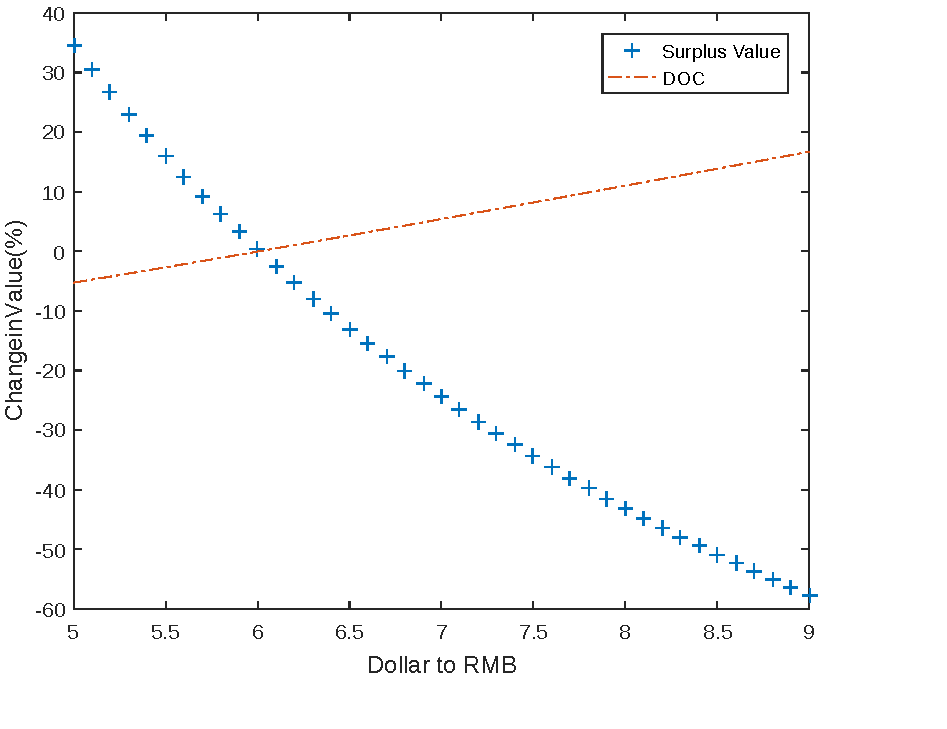
\includegraphics[width=3.2in,height=2.66in]{./media512/image1.pdf}
	\end{Center}
\end{figure}


%%%%%%%%%%%%%%%%%%%% Figure/Image No: 1 Ends here %%%%%%%%%%%%%%%%%%%%

\par

\begin{Center}
图5-4 汇率变化对飞机经济性的影响
\end{Center}\par

\begin{Center}
Fig.5-4 Exchange rate sensitivity study 
\end{Center}\par

图5-4中,飞机的直接使用成本随着汇率的提升而增加,而剩余价值随着汇率的增加而下降。采用AEA的方法进行国内DOC的估算需要进行汇率的转化。这中间涉及的成本项目计算包括机组人员的工资,维修材料成本的计算,维修劳务成本的计算等。\par

	\item \textbf{航空燃油价格对飞机经济性的影响}\par

航空燃油价格处于时刻变动中,而飞机的燃油成本占据使用成本很大的比重,因此飞机的使用经济性对航空燃油价格十分敏感,航空燃油价格对飞机经济性的影响如图5-5所示。\par



%%%%%%%%%%%%%%%%%%%% Figure/Image No: 2 starts here %%%%%%%%%%%%%%%%%%%%

\begin{figure}[H]
	\begin{Center}
		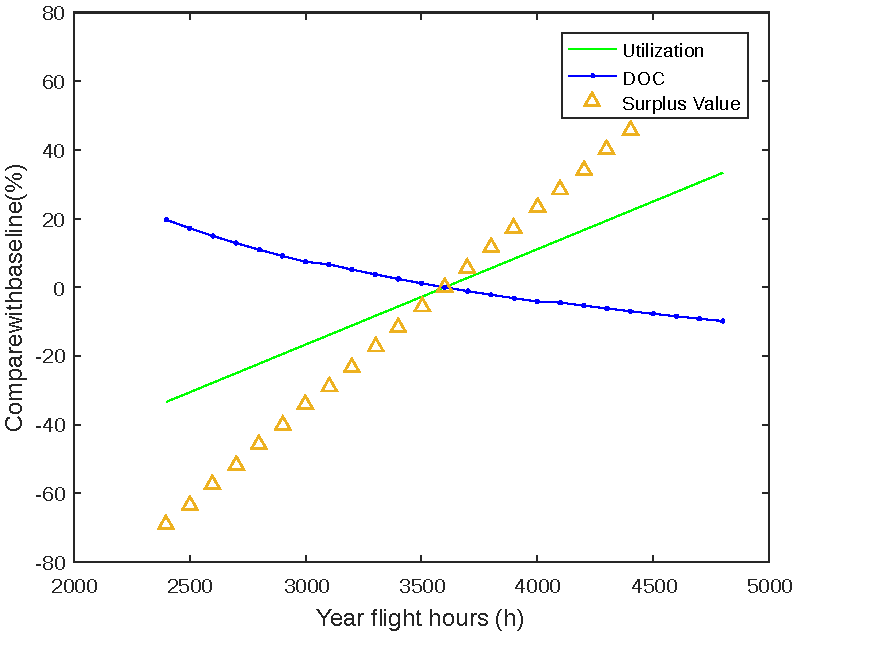
\includegraphics[width=3.74in,height=2.29in]{./media512/image2.pdf}
	\end{Center}
\end{figure}


%%%%%%%%%%%%%%%%%%%% Figure/Image No: 2 Ends here %%%%%%%%%%%%%%%%%%%%

\par

\begin{Center}
图5-5 航程与燃油价格对剩余价值的影响
\end{Center}\par

\begin{Center}
Fig.5-5 Flight distance ang fuel price impact on surplus value
\end{Center}\par


\vspace{\baselineskip}
图5-5中,飞机的剩余价值随着燃油成本的增加而下降,因为燃油成本的提升增加了飞机的使用成本,进而导致飞机的剩余价值下降。可以看到燃油价格的变化对飞机剩余价值产生显著的影响。\par



%%%%%%%%%%%%%%%%%%%% Figure/Image No: 3 starts here %%%%%%%%%%%%%%%%%%%%

\begin{figure}[H]
	\begin{Center}
		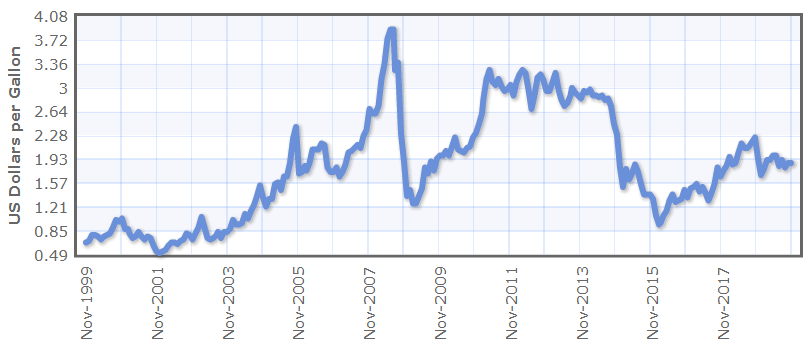
\includegraphics[width=5.04in,height=2.15in]{./media512/image3.png}
	\end{Center}
\end{figure}


%%%%%%%%%%%%%%%%%%%% Figure/Image No: 3 Ends here %%%%%%%%%%%%%%%%%%%%

\par

\begin{Center}
图5-6 近20年的燃油价格的变化\textsuperscript{[43]}
\end{Center}\par

\begin{Center}
Fig.5-6 Aviation fuel price in the past 20 years\textsuperscript{[43]}
\end{Center}\par

结合近20年航空燃油价格数据的剧烈波动,如图5-6所示。因此在飞机的设计过程中对飞机设计方案的经济性评估需要对航空燃油价格进行合理考虑。\par

	\item \textbf{物价上涨指数对飞机经济性的影响}
\end{enumerate}\par

物价上涨指数会影响飞机的研发成本与制造成本,物价上涨指数对飞机经济性的影响如图5-6所示。\par



%%%%%%%%%%%%%%%%%%%% Figure/Image No: 4 starts here %%%%%%%%%%%%%%%%%%%%

\begin{figure}[H]
	\begin{Center}
		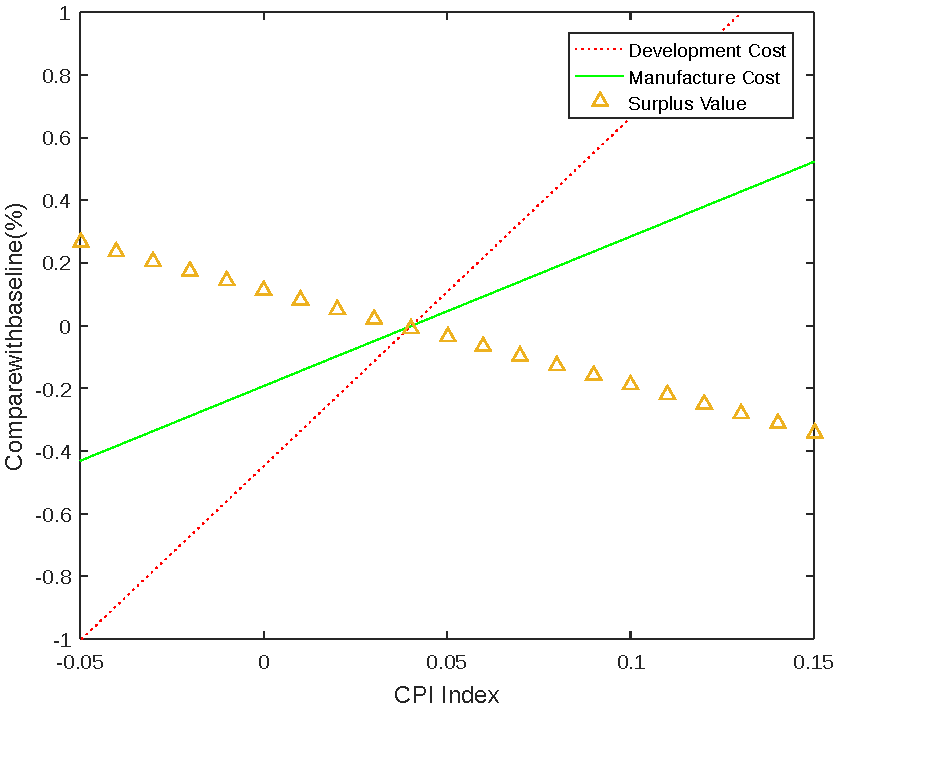
\includegraphics[width=3.17in,height=2.73in]{./media512/image4.pdf}
	\end{Center}
\end{figure}


%%%%%%%%%%%%%%%%%%%% Figure/Image No: 4 Ends here %%%%%%%%%%%%%%%%%%%%

\par

\begin{Center}
图5-7 物价上涨指数对飞机经济性的影响
\end{Center}\par

\begin{Center}
Fig.5-7 CPI impacts on aircraft economics
\end{Center}\par


\vspace{\baselineskip}
从图5-7可以看到,飞机的研发成本与制造成本随着物价上涨指数的增加而增加,因此飞机的剩余价值下降,物价上涨指数的增加并不利于飞机的经济性。\par

\subsubsection*{制造商生产参数的影响}
\addcontentsline{toc}{subsubsection}{制造商生产参数的影响}
飞机制造商的相关运营参数,包括飞机生产数量,飞机生产率,折扣率与折扣系数等参数,这些参数不会对飞机的参数产生直接影响,但是会影响相关的飞机设计属性,包括飞机的经济性,进而影响对飞机设计方案的权衡。\par

\begin{enumerate}
	\item \textbf{生产数量的影响}\par

 \ \  飞机的单击成本随着产量的增加而下降,飞机制造商只有在到达一定的产量之后才会到达盈亏平衡点进而盈利。飞机的产量对经济性的影响如图5-8所示。\par



%%%%%%%%%%%%%%%%%%%% Figure/Image No: 5 starts here %%%%%%%%%%%%%%%%%%%%

\begin{figure}[H]
	\begin{Center}
		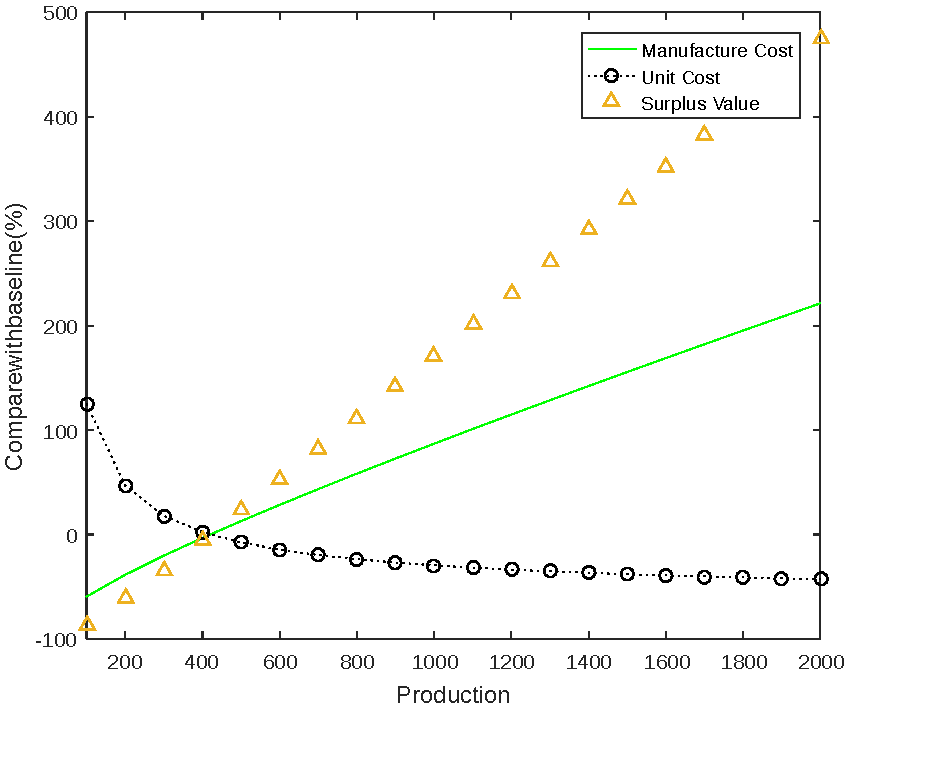
\includegraphics[width=3.59in,height=2.92in]{./media512/image5.pdf}
	\end{Center}
\end{figure}


%%%%%%%%%%%%%%%%%%%% Figure/Image No: 5 Ends here %%%%%%%%%%%%%%%%%%%%

\par

\begin{Center}
图 5-8产量对飞机经济性的影响
\end{Center}\par

\begin{Center}
Fig.5-8 Production impacts on aircraft economics
\end{Center}\par


\vspace{\baselineskip}
从图5-8可以得出,飞机的制造成本随着产量的增加而增加,而飞机的单机成本随产量的增加而减少,因为产量的提升均摊了固定成本。由于产量的提升以及单机成本的下降,飞机的剩余价值得以提升。\par

	\item \textbf{飞机制造商折扣率与投资期限的影响}
\end{enumerate}\par

公式(3-1)中剩余价值的计算需要考虑飞机制造商的折扣系数以及航空公司的折扣系数,折扣系数直接影响了飞机的剩余价值,而折扣率与投资期限则通过影响飞机的折扣率进而改变飞机的剩余价值。其中制造商与投资期限对剩余价值的影响如图5-9所示。\par



%%%%%%%%%%%%%%%%%%%% Figure/Image No: 6 starts here %%%%%%%%%%%%%%%%%%%%

\begin{figure}[H]
	\begin{Center}
		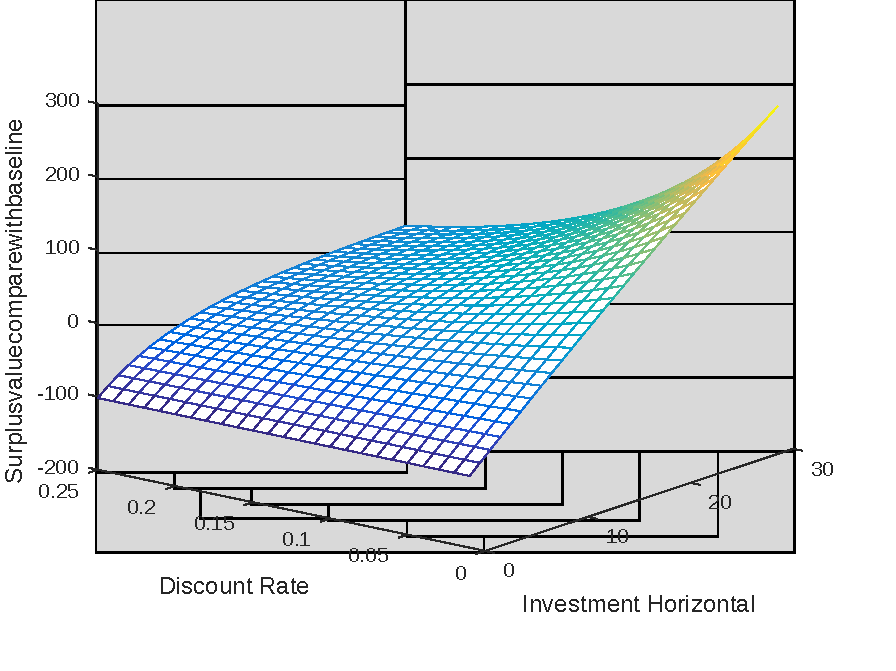
\includegraphics[width=3.9in,height=2.93in]{./media512/image6.pdf}
	\end{Center}
\end{figure}


%%%%%%%%%%%%%%%%%%%% Figure/Image No: 6 Ends here %%%%%%%%%%%%%%%%%%%%

\par

\begin{Center}
图5-9 飞机制造商的折扣率与投资期限对剩余价值的影响
\end{Center}\par

\begin{Center}
Fig.5-9 Discount rate and investment horizontal on aircraft economics
\end{Center}\par


\vspace{\baselineskip}
图5-9中,飞机的剩余价值同时受到折扣率与投资期限的影响,当飞机的折扣率较小时,飞机的剩余价值随着投资期限的增加而增加;当折扣率较大的时候,剩余价值随着投资期限的增加缓慢增加。\par

\subsubsection*{制造商设计活动相关参数的影响}
\addcontentsline{toc}{subsubsection}{制造商设计活动相关参数的影响}
飞机制造商与发动机制造商的相关设计活动参数会对飞机的经济性产生影响,这些设计活动相关参数包括飞机的FTA数量,相关设计的难度系数,材料系数等等。图5-10显示了制造商FTA数量对飞机经济性的影响。\par



%%%%%%%%%%%%%%%%%%%% Figure/Image No: 7 starts here %%%%%%%%%%%%%%%%%%%%

\begin{figure}[H]
	\begin{Center}
		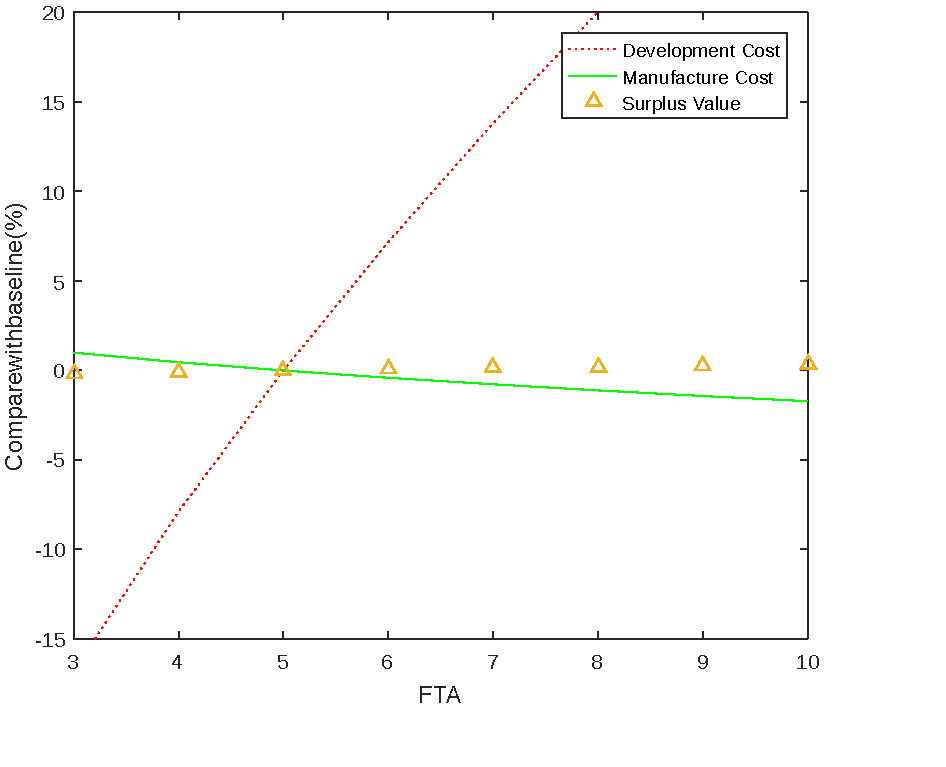
\includegraphics[width=3.72in,height=3.02in]{./media512/image7.pdf}
	\end{Center}
\end{figure}


%%%%%%%%%%%%%%%%%%%% Figure/Image No: 7 Ends here %%%%%%%%%%%%%%%%%%%%

\par

\begin{Center}
图5-10 FTA对飞机经济性的影响
\end{Center}\par

\begin{Center}
Fig.5-10 FTA impacts on aircraft economics
\end{Center}\par


\vspace{\baselineskip}
从图5-10可以知道,制造商的研发成本对FTA的数量变化十分敏感,飞机的研发成本随着飞机FTA数量的增加而增加,而制造成本随FTA的增加而减少,飞机的剩余价值对FTA数量的变化并不敏感,因为FTA的相关成本占SV的比重很小。\par


\vspace{\baselineskip}

\printbibliography
\end{document}